%%%%%%%%%%%%%%%%%%%%%%%%%%%%%%%%%%%%%%%%%%%%%%%%%%%%%%%%%%%%%%%%%%%%%%%%%%%%%%%%
%                                                                              %
%   2017 -- Diplomamunkavázlat                                                 %
%                                                                              %
%  A latex.feec.vutbr.cz weboldal által szolgáltatott minta alapján készült.   %
%  Importálva azok a csomagok lettek, melyek a mintában is vannak.             %
%                                                                              %
%%%%%%%%%%%%%%%%%%%%%%%%%%%%%%%%%%%%%%%%%%%%%%%%%%%%%%%%%%%%%%%%%%%%%%%%%%%%%%%%
\documentclass[a4paper, 12pt, unicode, czech]{report}
\usepackage[utf8]{inputenc}
\usepackage{graphicx}
\usepackage[nohyperlinks]{acronym}
\usepackage[breaklinks=true, hypertexnames=false]{hyperref}
\usepackage{pdfpages}
\usepackage{enumitem}
  \setlist{topsep=0pt,partopsep=0pt,noitemsep}
\usepackage{cmap}
\usepackage{upgreek}
\usepackage{dirtree}
\usepackage[formats]{listings}
\lstset{
% Definice jazyka použitého ve výpisech
% language=[LaTeX]{TeX},  % LaTeX
% language={Matlab},      % Matlab
  language={C},           % jazyk C
    basicstyle=\ttfamily, % definice základního stylu písma
    tabsize=2,            % definice velikosti tabulátoru
    inputencoding=utf8,   % pro soubory uložené v kódování UTF-8
    columns=fixed,        % flexible,
    fontadjust=true       % licovani sloupcu
    extendedchars=true,
    literate=             %  definice symbolů s diakritikou
    {á}{{\'a}}1
    {č}{{\v{c}}}1
    {ď}{{\v{d}}}1
    {é}{{\'e}}1
    {ě}{{\v{e}}}1
    {í}{{\'i}}1
    {ň}{{\v{n}}}1
    {ó}{{\'o}}1
    {ř}{{\v{r}}}1
    {š}{{\v{s}}}1
    {ť}{{\v{t}}}1
    {ú}{{\'u}}1
    {ů}{{\r{u}}}1
    {ý}{{\'y}}1
    {ž}{{\v{z}}}1
    {Á}{{\'A}}1
    {Č}{{\v{C}}}1
    {Ď}{{\v{D}}}1
    {É}{{\'E}}1
    {Ě}{{\v{E}}}1
    {Í}{{\'I}}1
    {Ň}{{\v{N}}}1
    {Ó}{{\'O}}1
    {Ř}{{\v{R}}}1
    {Š}{{\v{S}}}1
    {Ť}{{\v{T}}}1
    {Ú}{{\'U}}1
    {Ů}{{\r{U}}}1
    {Ý}{{\'Y}}1
    {Ž}{{\v{Z}}}1
}
\usepackage{nicefrac}   % szép törtek :) -- használata: \nicefrac{a}{b}, ami egy szép a/b formát fog adni
\usepackage{pgfplots}   % DIA-ból exportált ábrákhoz használt csomag használata.
\usepackage{listings}   % Forráskódok szedéséhez alkamazzuk ezt a csomagot.
\usepackage{babel}
\usepackage{lmodern}
\usepackage{textcomp}
\usepackage[T1]{fontenc}

\usepackage[%
%% Z následujících voleb lze použít pouze jednu
% left,               % Rovnice a popisky plovoucich objektů budou %zarovnány vlevo
  center,             % Rovnice a popisky plovoucich objektů budou zarovnány na střed (vychozi)
% Z následujících voleb lze použít pouze jednu
  semestral           % sazba zprávy semestrálního projektu
  %bachelor           % sazba bakalářské práce
  %diploma            % sazba diplomové práce
  %treatise           % sazba pojednání o dizertační práci
  %phd                % sazba dizertační práce
  ]{thesis}           % Balíček pro sazbu studentských prací
                      % Musí být vložen až jako poslední, aby
                      % ostatní balíčky nepřepisovaly jeho příkazy


%%%%%%%%%%%%%%%%%%%%%%%%%%%%%%%%%%%%%%%%%%%%%%%%%%%%%%%%%%%%%%%%%%%%%%%%%%%%%%%%
%                                                                              %
%   Paraméterek külső állományból való betöltése.                              %
%                                                                              %
%%%%%%%%%%%%%%%%%%%%%%%%%%%%%%%%%%%%%%%%%%%%%%%%%%%%%%%%%%%%%%%%%%%%%%%%%%%%%%%%
\autor[Bc.]{Péter}{Tóth}
\vedouci[Ing.]{Tomáš}{Urbanec }[Ph.D.]
\nazev{Název studentské práce}{Title of Student's Thesis}
%\oponent[doc.\ Mgr.]{Křestní}{Příjmení}[Ph.D.]
\oborstudia{Teleinformatika}{Teleinformatics}
\fakulta{Fakulta elektrotechniky a komunikačních technologií}{Faculty of Electrical Engineering and Communication}
\ustav{Ústav radioelektroniky}{Department of Radio Electronics}
\logofakulta[loga/FEKT_zkratka_barevne_PANTONE_CZ]{loga/UTKO_color_PANTONE_CZ}
\rok{2017}
\datum{19.\,12.\,2017} % Datum se uplatní pouze v prezentaci k obhajobě
\misto{Brno}
\abstrakt{Táto práce se zaobírá zpracováním přijatých signálů z amatérských družic NO-83 a NO-84 ParkinsonSat na nízké oběžné dráze (Low Earth Orbit – LEO) vysílajících telemetrické údaje v pásmu $70\,\mathrm{cm}$ vln. které jsou postiženy dopplerovským posuvem kmitočtu. Kvůli povaze oběžné dráhy a kmitočtu vysílání, přijatý signál je znatelně poškozen dopplerovským posuvem kmitočtu, který se musí kompenzovat pro pozdější potřeby demodulace.
}{This project work is dealing with processing of received radio signals of LEO satellites NO-83 and NO-84 ParkinsonSat transmitting in the 70--centimeter band. The nature of this kind of setup makes the received signal bearing a large amount of Doppler shift, which needs to be compensated in order to demodulate it.
}
\klicovaslova{korekce dopplerského posuvu, NO-83, BRICsat, NO-84, PSat, družice LEO, archiv dat TLE}
  {doppler shift correction, NO-83, BRICsat, NO-84, PSat, LEO satellites, TLE data archive}
\podekovanitext{Rád bych poděkoval vedoucímu diplomové práce panu Ing.~Tomášu Urbanci, Ph.D.\ za odborné vedení, konzultace, trpělivost a podnětné návrhy k~práci.}




%%%%%%%%%%%%%%%%%%%%%%%%%%%%%%%%%%%%%%%%%%%%%%%%%%%%%%%%%%%%%%%%%%%%%%%%%%%%%%%%
%                                                                              %
%   A diplomamunka vázlat szöveges részének kezdete.                           %
%                                                                              %
%%%%%%%%%%%%%%%%%%%%%%%%%%%%%%%%%%%%%%%%%%%%%%%%%%%%%%%%%%%%%%%%%%%%%%%%%%%%%%%%
\begin{document}
  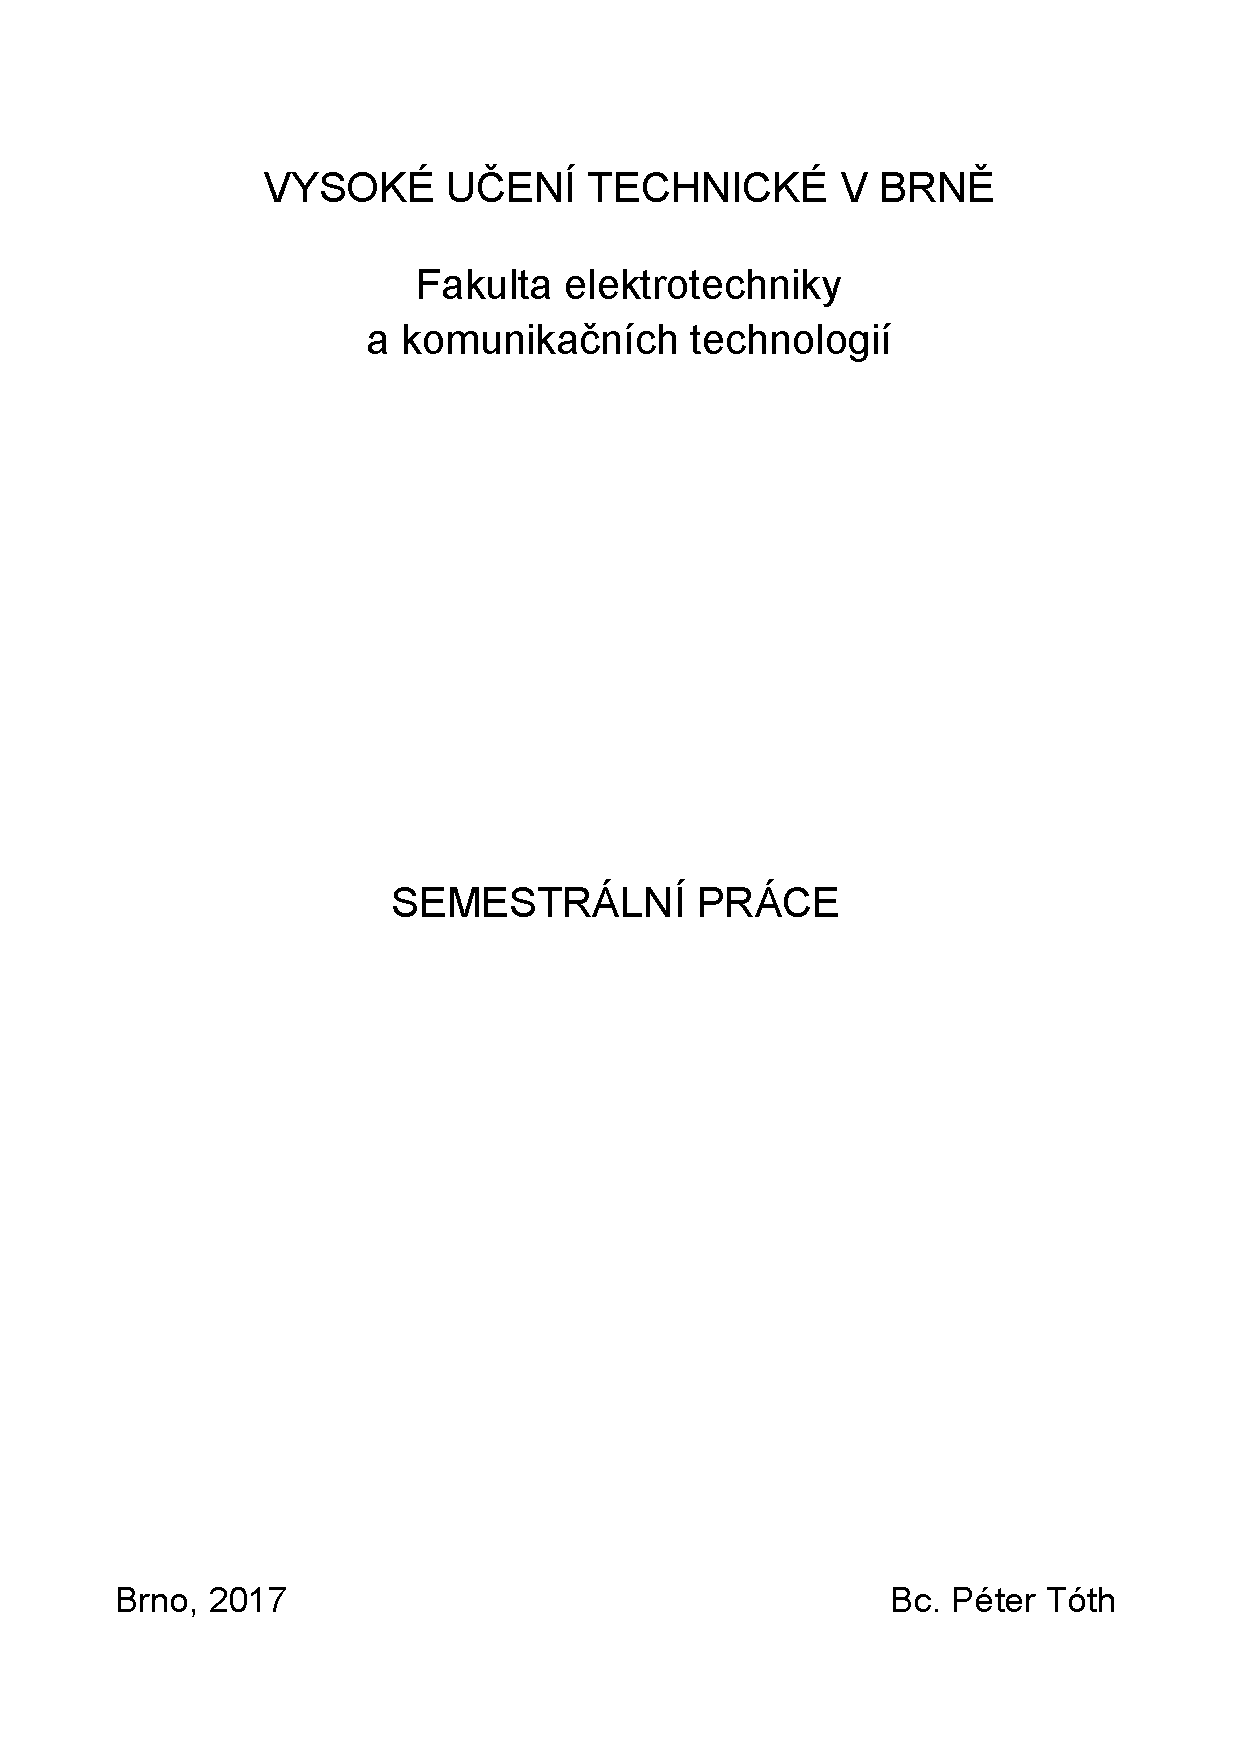
\includepdf[pages=1,offset=15.4mm -1in]{pdf/desky_xtothp00.pdf}     % Vložení desek generovaných informačním systémem
  \setcounter{page}{1}                                                % Resetovani citace stranek - desky se necisluji
  
\includepdf[pages=1,offset=15.4mm -1in]{pdf/titulni_list_cb.pdf}    % Vložení titulního listu generovaného informačním systémem
  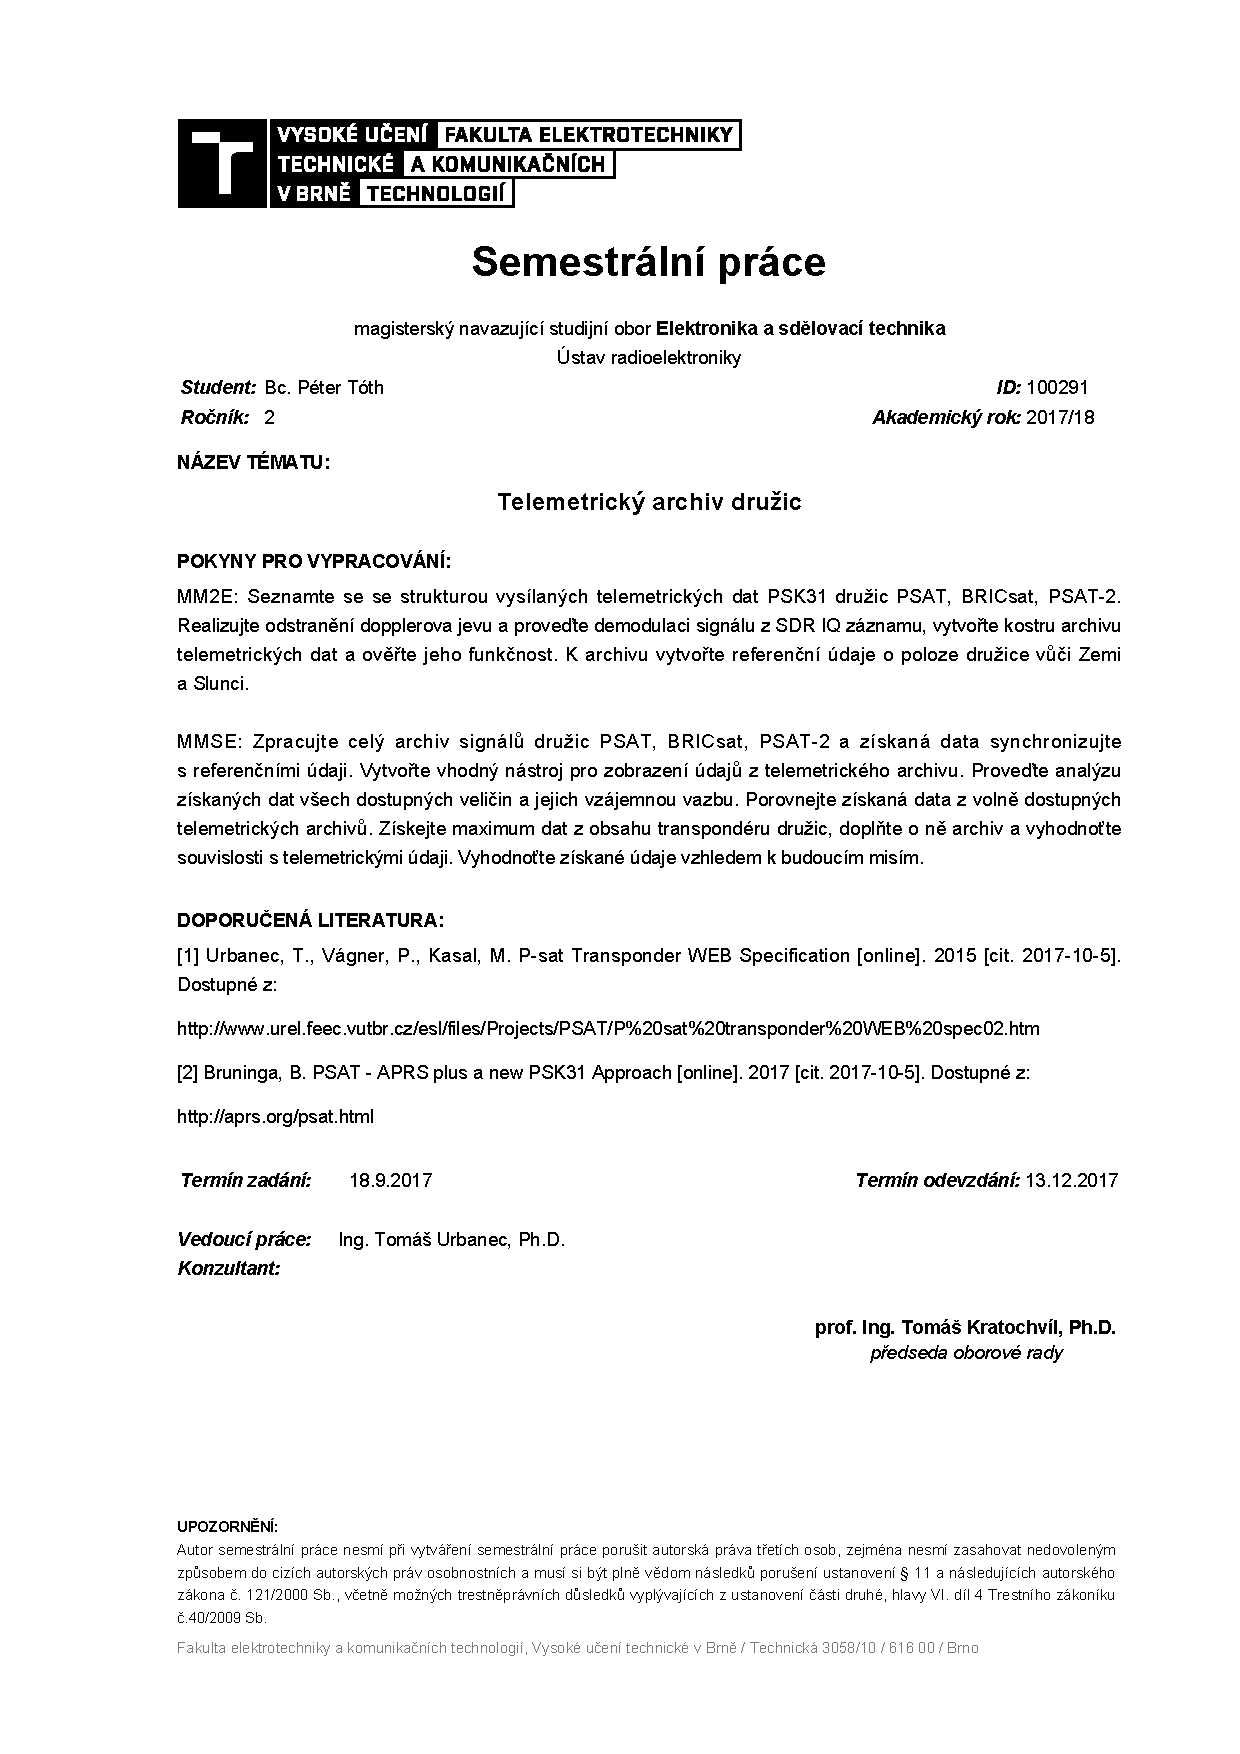
\includepdf[pages=1,offset=15.4mm -1in]{pdf/zadani_xtothp00_cb.pdf} % Vložení zadání generovaného informačním systémem

%%%%%%%%%%%%%%%%%%%%%%%%%%%%%%%%%%%%%%%%%%%%%%%%%%%%%%%%%%%%%%%%%%%%%%%%%%%%%%%%
% A tartalmi kivonat, köszönet rész.
  \vytvorabstrakt
  \vytvorprohlaseni
  \vytvorpodekovani

%%%%%%%%%%%%%%%%%%%%%%%%%%%%%%%%%%%%%%%%%%%%%%%%%%%%%%%%%%%%%%%%%%%%%%%%%%%%%%%%
% A tartalmak, felsorolások része.
  \obsah
  \seznamobrazku
  \seznamtabulek
  \lstlistoflistings

%%%%%%%%%%%%%%%%%%%%%%%%%%%%%%%%%%%%%%%%%%%%%%%%%%%%%%%%%%%%%%%%%%%%%%%%%%%%%%%%
% Az érdemi szöveg itt kezdődik.
  \chapter*{Úvod}
\phantomsection
\addcontentsline{toc}{chapter}{Úvod}

Umělé družice obíhající kolem Země jsou systémy, s kterými poslední fyzické kontakty lidí vznikají těsně před její vypuštěním. Prakticky to znamená praktickou nemožnost provádění jakékoliv činnosti na zařízení v místě působení činnosti umělé družice. Proto hraje důležitou roli při provozování umělých družic  dálkový sběr naměřených údajů senzorů, tzv. telemetrických dat, umělých družic za účelem vyhodnocení její stavu.

V této práci je vytvářená snaha o automatické zpracování telemetrických dat amatérských umělých družic Parkinson NO-83 a NO-84. Protože tyto družice mají svou dráhu na nízké oběžné dráze, je jejich signál silně postižen dopplerovským posuvem. Pro správní demodulaci signálu se tento posuv kmitočtu signálu musí korigovat, a kvůli číslicové povaze modulovaného signálu musí být táto korekce prováděná bez vzniku fázové diskontinuity.

Dělení dokumentu do kapitol a podkapitol je tvořen ze záměrem porozumění a sledování vzniku řešení zadaného a problému. Ke kompenzaci dopplerovského posuvu kmitočtu signálu musíme znát relativní rychlost družice vzhledem ke pozemní stanici. Pro výpočet této rychlosti musíme znát naši polohu, predikovat pohyb umělé družice a tvar její dráhy. Struční úvod do této problematiky na popsán v úseku \ref{sec:position}. V následující úseku \ref{sec:doppler} se věnujeme výpočtu relativní rychlosti umělé družice vzhledem k pozemní stanici nutnou pro výpočet velikosti dopplerovského posuvu.

V kapitole \ref{chap:python3} se prezentuje konkrétní řešení, včetně vývojových diagramů a popisu fungování jednotlivých skript v jazyce Python 3.

V příloze jsou uvedeny zdrojové kódy prezentovaných modulů.

  \chapter{Teorie}
\section[Struční přehled amaterských družic]{Struční přehled\\ amaterských družic}

Radiokomunikace prošla ohromným vývojem v průběhu druhé polovice 20. století. Vypuštění první umělé družice Sputnik-1 v roce 1957 datujeme začátek vesmírného věku. Od té doby se otevřeli nové možnosti radioamatérův věnovat se svému koníčku, nebo výzkumu.

    Necelé čtyři roky po vypuštění první umělé družice Země se svět dočkal první amatérské umělé družice sestrojeného v rámci projektu \zkratka{OSCAR} \cite{wiki:amateur_sat}, kterého nástupnickou organizaci se stal \zkratka{AMSAT} \cite{wiki:AMSAT}. Družice OSCAR I byla vypuštěná na nízkou oběžnou dráhu jako druhotný náklad, který vyžíval rezervy nosnosti rakety  Thor DM-21 Agena-B. Tento způsob dopravy byl zvolen z ekonomických důvodů a je dodnes používán.

    Obecně se amatérské družice nasazují na nízkou oběžnou dráhu (Low Earth Orbit -- LEO) \cite{book:ARRL_handbook}. Výhodou dráhy tohoto typu je jejich finanční nenáročnost, co je zčásti způsobená vlastností plynoucího z nazvu oběžné dráhy, výškou orbitu, který se pohybuje od $300\,\mathrm{km}$ do $2000\,\mathrm{km}$. Nedostatkem nízké oběžné dráhy je vysoká relativní rychlost družice vůči pozemní stanici, která přibližně $7{,}8\,\mathrm{\nicefrac{km}{s}}$ \cite{wiki:LEO} jehož důsledkem je rádiový signál značně postižen dopplerovským posuvem kmitočtu, kterého velikost dosahuje i $26\,\mathrm{ppm}$.



\section{Sledování a predikce pohybu těles na oběžné dráze Země}

Objekty, které se pohybují vesmírem kolem Země jsou sledovány organizacemi \cite{wiki:derbis}:
\begin{itemize}
    \item \zkratka{USSTRATCOM}(součást \zkratka{DoD})
    \item \zkratka{ESA}
    \item \zkratka{Fraunhofer-FHR}
    \item \zkratka{JPL}(součast \zkratka{NASA})
    \item \zkratka{MIT}
    \item \zkratka{EISCAT}
    \item \zkratka{USAF}
\end{itemize}

Ke sledování se používají pozemní radary, lidary, pozemní  a vesmírné teleskopy. Mezi sledované objekty patří umělé družice, pozůstatky raket a jiný vesmírný odpad. Nejrozsáhlejší katalog stavu družic udržuje Ministerstvo obrany Spojených států (\zkratka{DoD}) s názvem Space Object Catalog. Civilní varianta této databáze je provozována organizaci \zkratka{NASA}. Tyto databáze se udržují pomocí různých modelů orbitální mechaniky. Pohyby družic jsou analyticky vypočteny pomocí teorie všeobecných perturbací. Prvky dráhy této teorie jsou publikovány ve formátu \zkratka{NASA}/NORAD \zkratka{TLE}. \cite{wiki:US_space_surv}.

Proč se zabývat přesnou polohou družice? Aby jsme byly schopní provést korekci dopplerovského posuvu, musíme splnit několik požadavek výpočtu:
\begin{itemize}
%  \item přesný čas
  \item polohu pozemní stanice \footnote{pozemní stanici považujeme za stacionární vzhledem ke povrchu Země}
  \item polohu a rychlost umělé družice
\end{itemize}

%Pro korekci dopplerovského posuvu frekvence musíme znát polohu naši pozemní stanice, polohu družice a předpovědět její polohu. K tomu pozdějšímu nám právě napomáhají prvky dráhy ze souborů \zkratka{TLE} využívajíc model \zkratka{SGP4} \cite{wiki:TLE}.

\section{Výpočet rychlosti těles na oběžní dráze Země}
  Rychlost těles na oběžné dráze dráze lze precizně vypočítat pomocí vztahu \cite{wiki:orb_speed}:

  \begin{equation}
    v = \sqrt{\mu - \left( \frac{2}{r} - \frac{1}{a} \right)}
  \end{equation}

  kde $\mu$ je standardní gravitační parametr, $v$ je rychlost tělesa, $r$ je vzdálenost tělesa od místa pozorování, $a$ je délka hlavní poloosy.

  \begin{table}[ht]
    \begin{tabular}{l | c c }
      orbita        & výška orbitu     & rychlost orbitu                        \\
      $[-]$         & $[\mathrm{km}]$  & $[\nicefrac{\mathrm{km}}{\mathrm{s}}]$ \\
      \hline
      LEO           & $200$ -- $2000$  & $6{,}9$ -- $7{,}8$ pro kruhovou dráhu  \\
      Molnija       & $500$ -- $39900$ & $6{,}5$ -- $8{,}2$ pro eliptickou dráhu\\
      Geostacinární & $35768$          & $0{,}97$ -- $1{,}08$
    \end{tabular}
    \caption{Tangenciální rychlost pro různé orbity \cite{wiki:orb_speed}}
  \end{table}

\section{Určení dopplerovského posuvu}
  Pozorovatel, který je v relativním pohybu vzhledem ke zdroji vlnění, bude vnímat vlnění se změněným kmitočtem. V případě, že relativní rychlost se mění časem, mění se i velikost změny kmitočtu. Tuto změnu kmitočtu nazýváme dopplerovským posuvem a jev se nazývá Dopplerův jev, který byl publikovaný Christianem Dopplerem v roce 1842 v Praze.

  Velikost dopplerovského posuvu lze přibližně určit pomocí vztahu \cite{wiki:doppler_effect}:
  \begin{equation}
    \Delta f = \frac{\Delta v}{c} f_0
  \end{equation}

  kde $\Delta f$ je posuv kmitočtu, $\Delta v$ je relativní rychlost, $c$ rychlost vln v prostředí, $f_0$ je původní kmitočet.

  Pro výpočet dopplerovského posuvu signálu vysílaného družicí na oběžné dráze Země je potřebné znát její relativní rychlost vzhledem k pozorovateli na pozemní stanici. Tuto rychlost lze vypočítat z oběžné rychlosti družice pomocí trigonometrických výpočtů. Princip je zobrazen na obrázku \ref{img:rel_vel}
  \begin{figure}[ht]
    \centering
    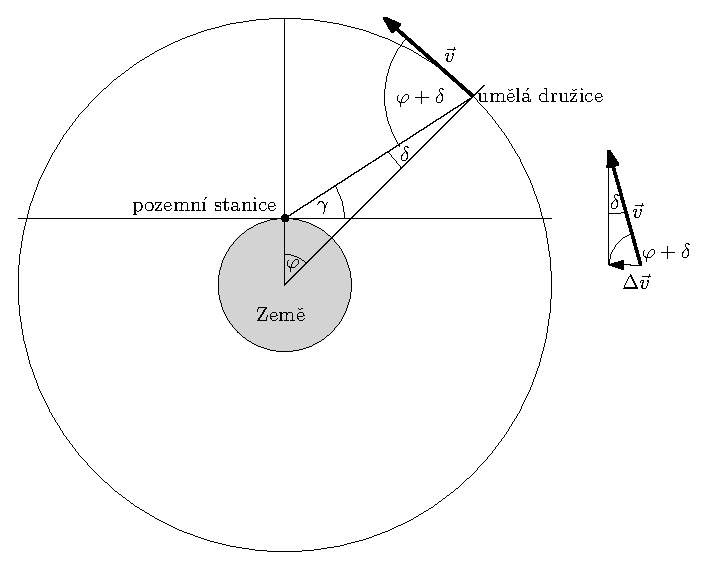
\includegraphics{./obrazky/doppler_shift.eps}
    \caption{Výpočet vektoru relatívní rychlosti \cite{book:doppler_compensation}}
    \label{img:rel_vel}
  \end{figure}


%\chapter{Korekce dopplerovského posuvu}
%  TBD\dots
%
%\chapter{Demodulace a dekódování signálu}
%  TBD\dots

  \chapter{vytvoření archivu dat TLE}
  Vytvoření lokální databázi dat TLE je nezbytné pro správnou korekci dopplerovského posuvu. Pro umělé družice NO-83 a NO-84 jsou veřejně přístupné data TLE na stránce organizace \zkratka{AMSAT}: <\url{http://amsat.org/pipermail/keps/}>. Tyto data jsou distribuované formou elektronického mailing list, kterého archív se nachází na výše zmíněném URL v jedním souboru. Aby bylo možné použit údaje TLE obsáhnuty v tomhle archivním souboru, je nutné provést extrakci dat TLE dle datu jejího vzniku.

  Na obrázku \ref{fig:TLE_flow} je uveden vývojový diagram skriptu pro extrahování dat TLE. Jako povinný vstupní parametr je název souboru staženého z webové stránky oragnizace \zkratka{AMSAT}. Data TLE jsou posílané v jednom emailu. Skript identifikuje začátek i konec balíků dat TLE. Na začátku každého balíku se hledjí vzory:\\
  \texttt{SB\textbackslash s+KEPS\textbackslash s+@\textbackslash s+AMSAT\textbackslash s+\$ORB\textbackslash d{5}\textbackslash.[A-Z]}\\
  \texttt{\textasciicircum 2Line}\\
  pomocí nástroje na vyhledávání regulárních výrazů implementovaného modulem re ze standardní knihovny jazyka Python. Konec bálíka je značen řetězcem
  \texttt{\textbackslash EX}.

  V případě, že skript narazí na hledaný výraz, nastaví se příslušný příznak. Tyto příznaky zaručí, aby řádky jednoho balíku se připojili k jednomu řetězci. Když skript identifikuje poslední řádek, pospojovaný řetězec řádků se připojí k množině všech balíků TLE dat. Návratovou hodnotou je právě tato množina. Množina v jazyce Python 3 zaručuje jedinečnost všech prvků, obdobně jako množiny z teorie množin.

  K výpisu souboru patří funkce \texttt{dump\_to\_file} skriptu \texttt{TLE.py}. Tato funkce má jeden povinný parametr, množinu dat TLE. Z této množiny se načte každý jeden prvek. V těchto prvcích se prohledává datum vzniku, což se použije jako název souboru. Následně se dle potřeby vytvoří adresář, kterého název je rok vzniku TLE dat. Před vytvářením adresáře se kontroluje přítomnost adresáře, nebo souboru stejného jména, jaký se chystá být vytvořit. Jestli adresář se stejným jménem existuje, začne se de ní zapisovat. V opačném případě předpokládáme, že v adresáři je soubor se stejný jménem musíme název složky, kterou se chystáme vytvořit změnit z důvodu nemožnosti koexistence souboru a adresáře stejného jména v rodičovském adresáři. K názvu složky se přidává znak podtržítka a číslo, které se iteruje inkrementací do doby, kdy v rodičovském se nebude nacházet soubor se stejným jménem. V případě adresáře se stejným jménem nalezeného po přidání dodatečných znaků k názvu souboru, se adresář začne používat k uložení souborů. Čtení z množiny je realizováno pomocí iterací nad její prvkami.

%  ../../Python3/TLE.py
  \begin{figure}[ht]
    \centering
    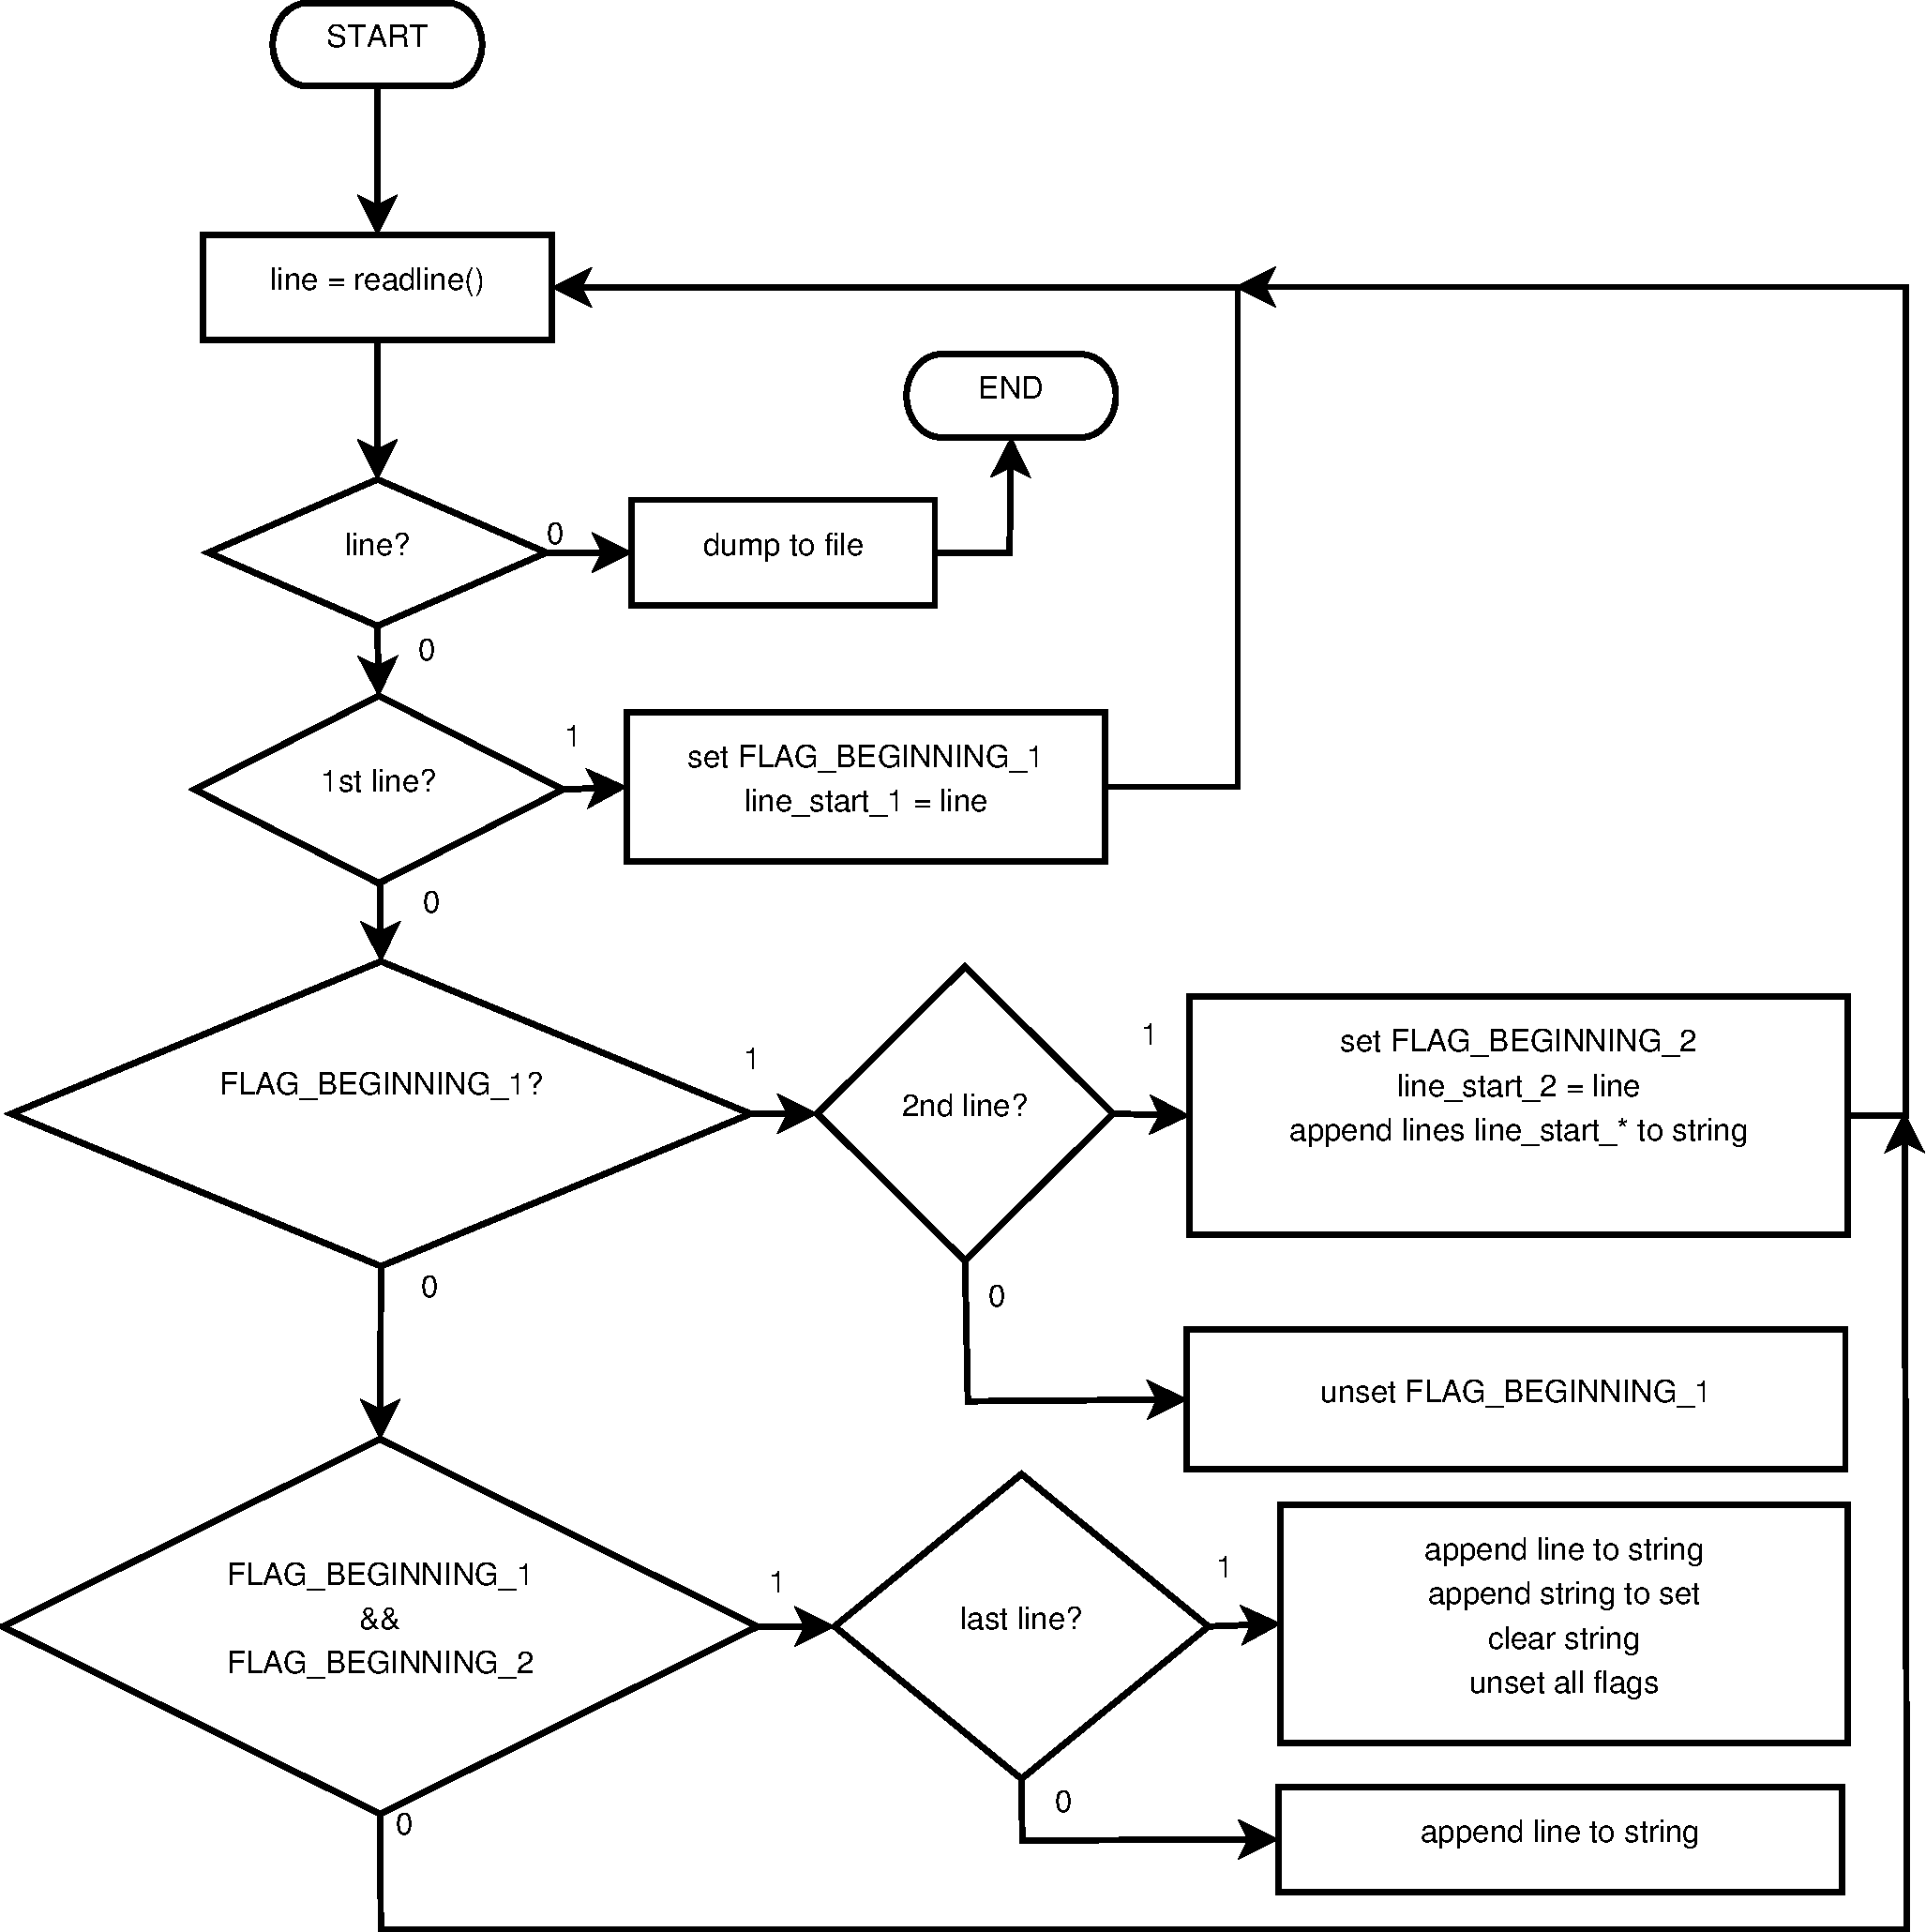
\includegraphics[width=0.98\textwidth]{./obrazky/TLE.pdf}
    \caption{Vývojový diagram extrahování dat TLE}
    \label{fig:TLE_flow}
  \end{figure}

\chapter{Korekce dopplerovského posuvu}
% gpredict -- libgpredict, doppler
% mediainfo, sox
  Po úspěšném získání nutných souborů s daty TLE pro umělé družice našeho zájmu, můžeme přistoupit ke korekci dopplerovského posuvu signálu, kterou provedeme pomocí programu doppler volně dostupného z repozitáře GIT týmu codehub dostupného na URL <\url{https://github.com/cubehub}>.

  Program doppler je utlitou příkazového řádku, který ze standardního vstupu čte IQ (in-phase, quadrature) data a zpracovává dle zadaných parametrů. Rozlišujeme dva režimy korekce frekvenčního posuvu. V režimu \emph{const} se kompenzuje konstantní posuv kmitočtu, kým v režimu \emph{track} se provádí korekce sledováním pohybu umělé družice a to i dodatečně v případě zpracování předem zaznamenaných dat IQ. V pozdním případě se programu doppler musí předát argument datu a času záznamu ve formátu ISO 8601 \cite{wiki:timeISO} \cite{github:doppler} bez udání časového posuvu v čase UTC.

  Korekce dopplerovského posuvu se provádí programem doppler za pomoci volně dostupné knihovny libgpredict, který je založen na predikčním kódu programu Gpredict\cite{github:ligpredict}

  Aby se zjednodušilo zpracování velikého množství souborů, byl vytvořen skript v jazyce Python 3 pro automatické zpracování záznamů s IQ daty. Modul get\_undopplred má definovanou funkci undoppler\_it, který jako vstupní parametry má:
  \begin{itemize}
    \item název souboru IQ dat
    \item název družice v notaci OSCAR\footnote{v našém případě se jedná o NO-83, NO-84}
    \item kmitočet na kterém je z družice vysíláno
    \item adresář s IQ daty
    \item adresář s TLE daty
    \item lokace pozemní stanice
  \end{itemize}

  Pomocí těchto údajů se sestrojí řetězec obsahující příkaz shellu BASH, kde jednotlivé příkazy jsou řazeny do tzv. kolony. Jde o zřetězení příkazů oddělených metaznakem svislá čára '|'. Standardní výstup příkazu se předává standardnímu příkazu následujícímu. \cite{book:Brandejs-unix-linux}

  Parametry záznamu IQ dat se zjišťují pomocí modulu pymediainfo, který je tzv. wrapper function knihovny Mediainfo \cite{github:pymediainfo}. Pomocí tohoto modelu lze zjistit kmitočet vzorkování, bitovou hloubku, kódování, počet kanálů, kodek.

  Aby jsme mohli soubory formátu \zkratka{WAV} použít jako vstupní data pro program doppler, je nutné provést změnu formátu dle očekávání programu. K této úloze se použije volný program \zkratka{sox}. Podobně na výstupu lze použít \zkratka{sox} pro převod z RAW Audio formátu na \zkratka{WAV}.

  \begin{figure}[ht]
    \centering
    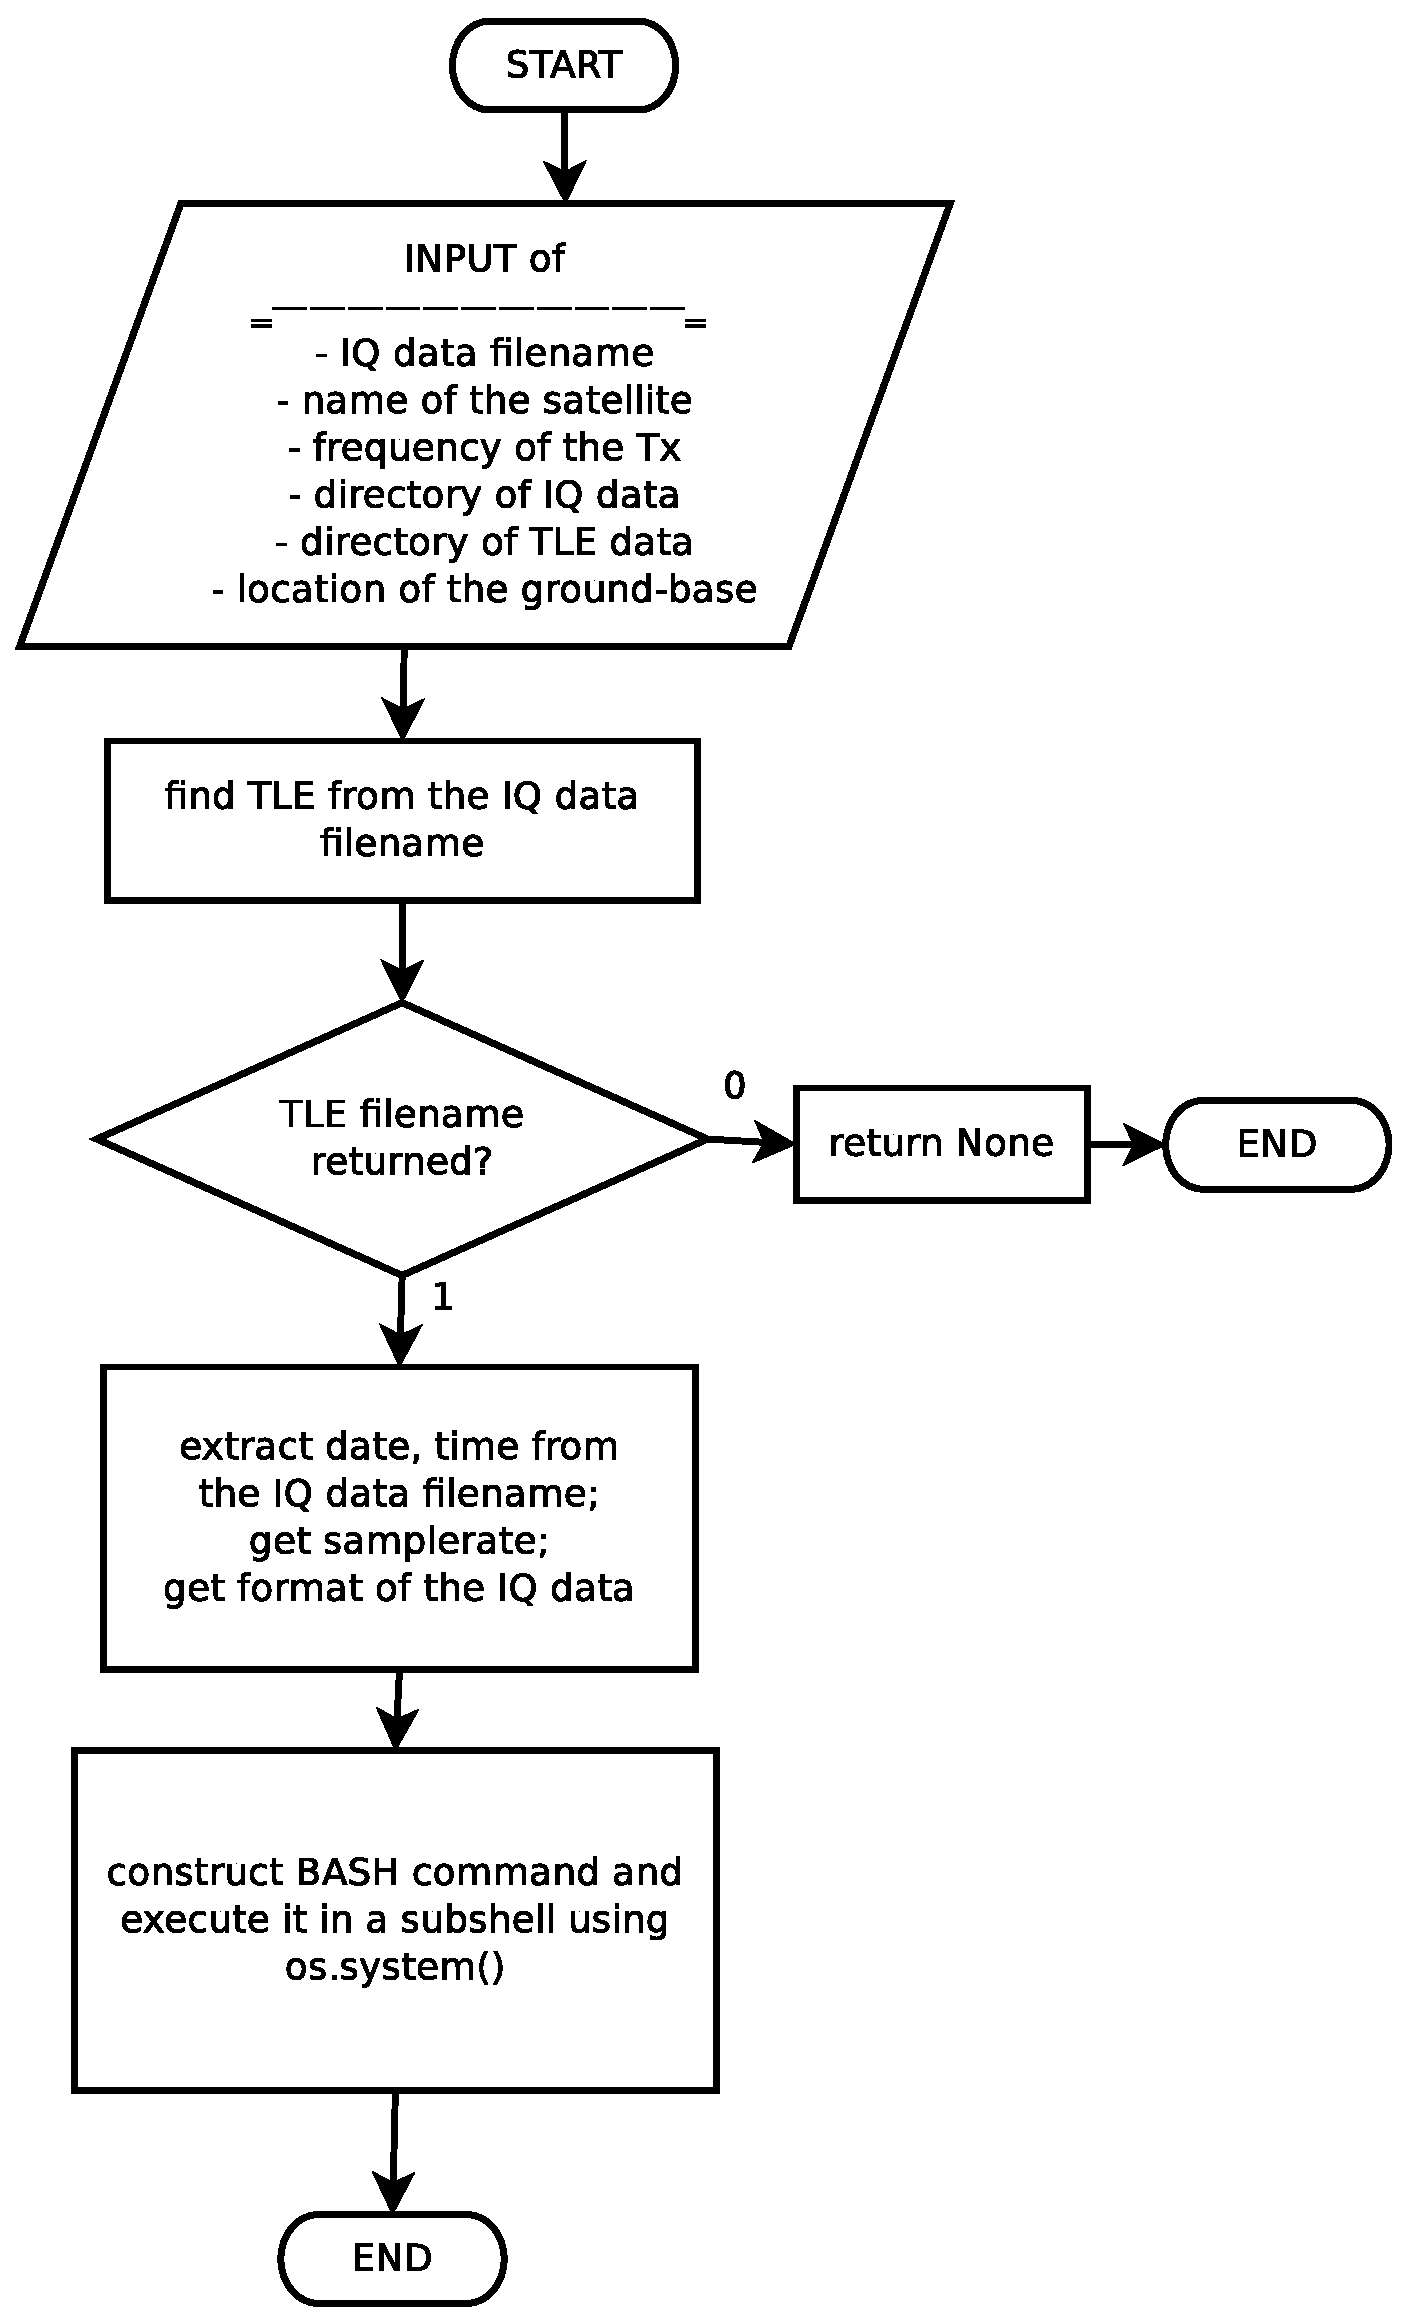
\includegraphics[width=0.65\textwidth]{./obrazky/get_undopplered.eps}
    \caption{Náčrt fungování modulu pro korekci dopplerovho posuvu}
    \label{fig:undoppler}
  \end{figure}

  \chapter{Závěr}
  TBD\dots

  % Pro sazbu seznamu literatury použijte jednu z následujících možností

%%%%%%%%%%%%%%%%%%%%%%%%%%%%%%%%%%%%%%%%%%%%%%%%%%%%%%%%%%%%%%%%%%%%%%%%%
%1) Seznam citací definovaný přímo pomocí prostředí literatura / thebibliography

\begin{literatura}{99}

\bibitem{wiki:amateur_sat}
    \emph{Amateur radio satellite}. In: Wikipedia: the free encyclopedia\/ [online].
    San Francisco (CA): Wikimedia Foundation, 2001- [cit. 2017-12-10].
    Dostupné z~URL:\\
    <\url{https://en.wikipedia.org/wiki/Amateur_radio_satellite}>.

\bibitem{wiki:AMSAT}
    \emph{Amateur radio satellite}. In: Wikipedia: the free encyclopedia\/ [online].
    San Francisco (CA): Wikimedia Foundation, 2001- [cit. 2017-12-10].
    Dostupné z~URL:\\
    <\url{https://en.wikipedia.org/wiki/AMSAT}>.

\bibitem{book:ARRL_handbook}
    PUBLISHED BY AMERICAN RADIO RELAY LEAGUE.
    \emph{The ARRL handbook for radio communications 2011.} 88th ed. Newington, CT: American Radio Relay League, 2010. ISBN 9780872590953.

\bibitem{wiki:LEO}
    \emph{Low Earth orbit}. In: Wikipedia: the free encyclopedia\/ [online].
    San Francisco (CA): Wikimedia Foundation, 2001- [cit. 2017-12-10].
    Dostupné z~URL:\\
    <\url{https://en.wikipedia.org/wiki/Low_Earth_orbit}>.

\bibitem{wiki:derbis}
    \emph{Space derbis}. In: Wikipedia: the free encyclopedia\/ [online].
    Dostupné z~URL:\\
    <\url{https://en.wikipedia.org/wiki/Space_debris}>.

\bibitem{wiki:US_space_surv}
    \emph{United States Space Surveillance Network}. In: Wikipedia: the free encyclopedia\/ [online].
    Dostupné z~URL:\\
    <\url{https://en.wikipedia.org/wiki/United_States_Space_Surveillance_Network}>.

\bibitem{wiki:TLE}
    \emph{Two-line element set}. In: Wikipedia: the free encyclopedia\/ [online].
    Dostupné z~URL:\\
    <\url{https://en.wikipedia.org/wiki/Two-line_element_set}>.

\bibitem{wiki:timeISO}
    \emph{ISO 8601}. In: Wikipedia: the free encyclopedia\/ [online].
    Dostupné z~URL:\\
    <\url{https://en.wikipedia.org/wiki/ISO_8601}>.

\bibitem{github:doppler}
    \emph{Doppler documentation}. [online].
    Dostupné z~URL:\\
    <\url{https://github.com/cubehub/doppler}>.

\bibitem{github:libgpredict}
    \emph{Libgpredict documentation}. [online].
    Dostupné z~URL:\\
    <\url{https://github.com/cubehub/libgpredict}>.

\bibitem{book:Brandejs-unix-linux}
    BRANDEJS, Michal.
    \emph{UNIX - Linux: praktický průvodce.} Praha: Grada, 1996. ISBN 80-7169-170-4.

\bibitem{github:pymediainfo}
    \emph{Pymediainfo github repository}. [online].
    Dostupné z~URL:\\
    <\url{https://github.com/sbraz/pymediainfo}>.

\bibitem{book:doppler_compensation}
    Gerorge P. Ah-Thew
    \emph{Doppler compensation for LEO satellite communication systems}. [online]
    <\url{https://macsphere.mcmaster.ca/bitstream/11375/5713/1/fulltext.pdf}>.

%\bibitem{\cite{wiki:orb_speed}
%    \emph{Orbital speed}. In: Wikipedia: the free encyclopedia\/ [online].
%    Dostupné z~URL:\\
%    <\url{https://en.wikipedia.org/wiki/Orbital_speed}>.
\bibitem{wiki:orb_speed}
    \emph{Orbital speed}. In: Wikipedia: the free encyclopedia\/ [online].
    Dostupné z~URL:\\
    <\url{https://en.wikipedia.org/wiki/Orbital_speed}>.

\bibitem{wiki:doppler_effect}
    \emph{Orbital speed}. In: Wikipedia: the free encyclopedia\/ [online].
    Dostupné z~URL:\\
    <\url{https://en.wikipedia.org/wiki/Doppler_effect}>.

\bibitem{wiki:train}
    \emph{Land speed record for rail vehicles}. In: Wikipedia: the free encyclopedia\/ [online].
    Dostupné z~URL:\\
    <\url{https://en.wikipedia.org/wiki/Land_speed_record_for_rail_vehicles}>.

\bibitem{wiki:sqlite}
    \emph{SQLite}. In: Wikipedia: the free encyclopedia\/ [online].
    Dostupné z~URL:\\
    <\url{https://en.wikipedia.org/wiki/SQLite}>.

%\bibitem{CSN_ISO_690-2011}
%    \emph{ČSN ISO 690 (01 0197) Informace a dokumentace -- Pravidla pro bibliografické odkazy a citace informačních zdrojů.}
%    40 stran. Praha: Český normalizační institut, 2011.
%
%\bibitem{CSN_ISO_7144-1997}
%    \emph{ČSN ISO 7144 (010161) Dokumentace -- Formální úprava disertací a podobných dokumentů.}
%    24 stran. Praha: Český normalizační institut, 1997.
%
%\bibitem{CSN_ISO_31-11}
%    \emph{ČSN ISO 31-11 Veličiny a jednotky -- část 11: Matematické znaky a značky používané ve fyzikálních vědách a v~technice.}
%    Praha: Český normalizační institut, 1999.
%
%\bibitem{BiernatovaSkupa2011:CSNISO690komentar}
%    BIERNÁTOVÁ, O., SKŮPA, J.:
%    \emph{Bibliografické odkazy a citace dokumentů dle ČSN ISO 690 (01 0197) platné od 1.\,dubna 2011}\/ [online].
%    2011, poslední aktualizace 2.\,9.\,2011 [cit. 19.\,10.\,2011].
%    Dostupné z~URL:
%    \(<\)\url{http://www.citace.com/CSN-ISO-690.pdf}\(>\)
%%    \(<\)\href{http://www.boldis.cz/citace/citace.html}{http://www.boldis.cz/citace/citace.html}\(>\).
%
%\bibitem{pravidla}
%    \emph{Pravidla českého pravopisu}.
%    Zpracoval kolektiv autorů. 1.\ vydání.
%    Olomouc: FIN PUB\-LISH\-ING, 1998. 575 s. ISBN 80-86002-40-3.
%
%\bibitem{Walter1999}
%  WALTER, G.\,G.; SHEN, X.
%  \emph{Wavelets and Other Orthogonal Systems}.
%  2. vyd. Boca Raton: Chapman\,\&\,Hall/CRC, 2000. 392~s. ISBN 1-58488-227-1
%
%\bibitem{Svacina1999IEEE}
%  SVAČINA, J.
%  Dispersion Characteristics of Multilayered Slotlines -- a Simple Approach.
%  \emph{IEEE Transactions on Microwave Theory and Techniques},
%  1999, vol.\,47, no.\,9, s.\,1826--1829. ISSN 0018-9480.
%
%\bibitem{RajmicSysel2002}
%    RAJMIC, P.; SYSEL, P.
%    Wavelet Spectrum Thresholding Rules.
%    In \emph{Proceedings of the International Conference Research in Telecommunication Technology},
%    Žilina: Žilina University, 2002. s.\,60--63. ISBN 80-7100-991-1.

\end{literatura}


%%%%%%%%%%%%%%%%%%%%%%%%%%%%%%%%%%%%%%%%%%%%%%%%%%%%%%%%%%%%%%%%%%%%%%%%%
%%2) Seznam citací pomocí BibTeXu
%% Při použití je nutné v TeXnicCenter ve výstupním profilu aktivovat spouštění BibTeXu po překladu.
%% Definice stylu seznamu
%\bibliographystyle{unsrturl}
%% Pro českou sazbu lze použít styl czechiso.bst ze stránek
%% http://www.fit.vutbr.cz/~martinek/latex/czechiso.tar.gz
%%\bibliographystyle{czechiso}
%% Vložení souboru se seznamem citací
%\bibliography{text/literatura}
%
%% Následující příkaz je pouze pro ukázku sazby literatury při použití BibTeXu.
%% Způsobí citaci všech zdrojů v souboru odkazy.bib, i když nejsou citovány v textu.
%\nocite{*}

  \begin{seznamzkratek}{KolikMista}

  \novazkratka{AMSAT}                        % název
      {AMSAT-NA}                             % zkratka
      {Radio Amateur Satellite Corporation}  % rozvinutí zkratky

  \novazkratka{OSCAR}
      {OSCAR}
      {Orbiting Satellite Carrying Amateur Radio}

  \novazkratka{USSTRATCOM}
      {USSTRATCOM}
      {United States Strategic Command}

  \novazkratka{DoD}
      {DoD}
      {Department of Defense}

  \novazkratka{ESA}
      {ESA}
      {European Space Agency}

  \novazkratka{Fraunhofer-FHR}
      {Fraunhofer-FHR}
      {Fraunhofer-Institut fur Hochfrequenzphysik und Radartechnik}

  \novazkratka{TIRA}
      {TIRA}
      {Tracking \& Imaging Radar}

  \novazkratka{NASA}
      {NASA}
      {National Aeronautics and Space Administration}

  \novazkratka{JPL}
      {JPL}
      {Jet Propulsion Laboratory}

  \novazkratka{GDSCC}
      {GDSCC}
      {Goldstone Deep Space Communications Complex}

  \novazkratka{MIT}
      {MIT}
      {Massachusetts Institute of Technology}

  \novazkratka{EISCAT}
      {EISCAT}
      {European Incoherent Scatter Scientific Association}

  \novazkratka{USAF}
      {USAF}
      {United States Air Force}

  \novazkratka{TLE}
      {TLE}
      {two-line elements}

  \novazkratka{SGP4}
      {SGP4}
      {Simplified perturbations models}

  \novazkratka{UTC}
      {UTC}
      {Coordinated Universal Time}

  \novazkratka{WAV}
      {WAVE}
      {Waveform Audio File Format}

  \novazkratka{sox}
      {SoX}
      {Sound eXchange}

  \novazkratka{PNG}
      {PNG}
      {Portable Network Graphics}


%  %%% bsymfvz
%  \novazkratka{symfvz}            % název
%    {\ensuremath{f_\textind{vz}}} % symbol
%    {vzorkovací kmitočet}          % popis
%  %%% esymfvz

\end{seznamzkratek}


%%%%%%%%%%%%%%%%%%%%%%%%%%%%%%%%%%%%%%%%%%%%%%%%%%%%%%%%%%%%%%%%%%%%%%%%%%%%%%%%
% Csatolmányok
  \prilohy
  \seznampriloh
  \chapter{Některé příkazy balíčku \texttt{thesis}}

\section{Příkazy pro sazbu veličin a jednotek}

\begin{table}[!h]
  \caption{Přehled příkazů pro matematické prostředí }
  \begin{center}
  	\small
	  \begin{tabular}{|c|c|c|c|}
	    \hline
	    Příkaz    						& Příklad 					& Zdroj příkladu  							& Význam  \\
	    \hline\hline
	    \verb|\textind{...}|	& $\beta_\textind{max}$ 	& \verb|$\beta_\textind{max}$|	& textový index \\
	    \hline
	    \verb|\konst{...}| 		& $\konst{U}_\textind{in}$ 				& \verb|$\konst{U}_\textind{in}$|		& konstantní veličina \\
	    \hline
	    \verb|\prom{...}| 		& $\prom{u}_\textind{in}$ & \verb|$\prom{u}_\textind{in}$| & proměnná veličina \\
	    \hline
	    \verb|\komplex{...}| 	& $\komplex{u}_\textind{in}$ & \verb|$\komplex{u}_\textind{in}$| & komplexní veličina \\
	    \hline
	    \verb|\vekt{...}| 		& $\vekt{y}$ 						& \verb|$\vekt{y}$| & vektor \\
	    \hline
	    \verb|\matice{...}| 	& $\matice{Z}$ 						& \verb|$\matice{Z}$| & matice \\
	    \hline
	    \verb|\jedn{...}| 		& $\jedn{kV}$ 						& \verb|$\jedn{kV}$|\quad či\ \, \verb|\jedn{kV}| & jednotka \\
	    \hline
	  \end{tabular}
  \end{center}
\end{table}



%\newpage
\section{Příkazy pro sazbu symbolů}

\begin{itemize}
  \item
    \verb|\E|, \verb|\eul| -- sazba Eulerova čísla: $\eul$,
  \item
    \verb|\J|, \verb|\jmag|, \verb|\I|, \verb|\imag| -- sazba imaginární jednotky: $\jmag$, $\imag$,
  \item
    \verb|\dif| -- sazba diferenciálu: $\dif$,
  \item
    \verb|\sinc| -- sazba funkce: $\sinc$.
  \item
    \verb|\mikro| -- sazba symbolu mikro stojatým písmem\footnote{znak pochází z~balíčku \texttt{textcomp}}: $\mikro$.

\end{itemize}
%
Všechny symboly jsou určeny pro matematický mód, vyjma \verb|\mikro|, jenž je\\ použitelný rovněž v~textovém módu.






\chapter{Druhá příloha}

\begin{figure}[!h]
  \begin{center}
    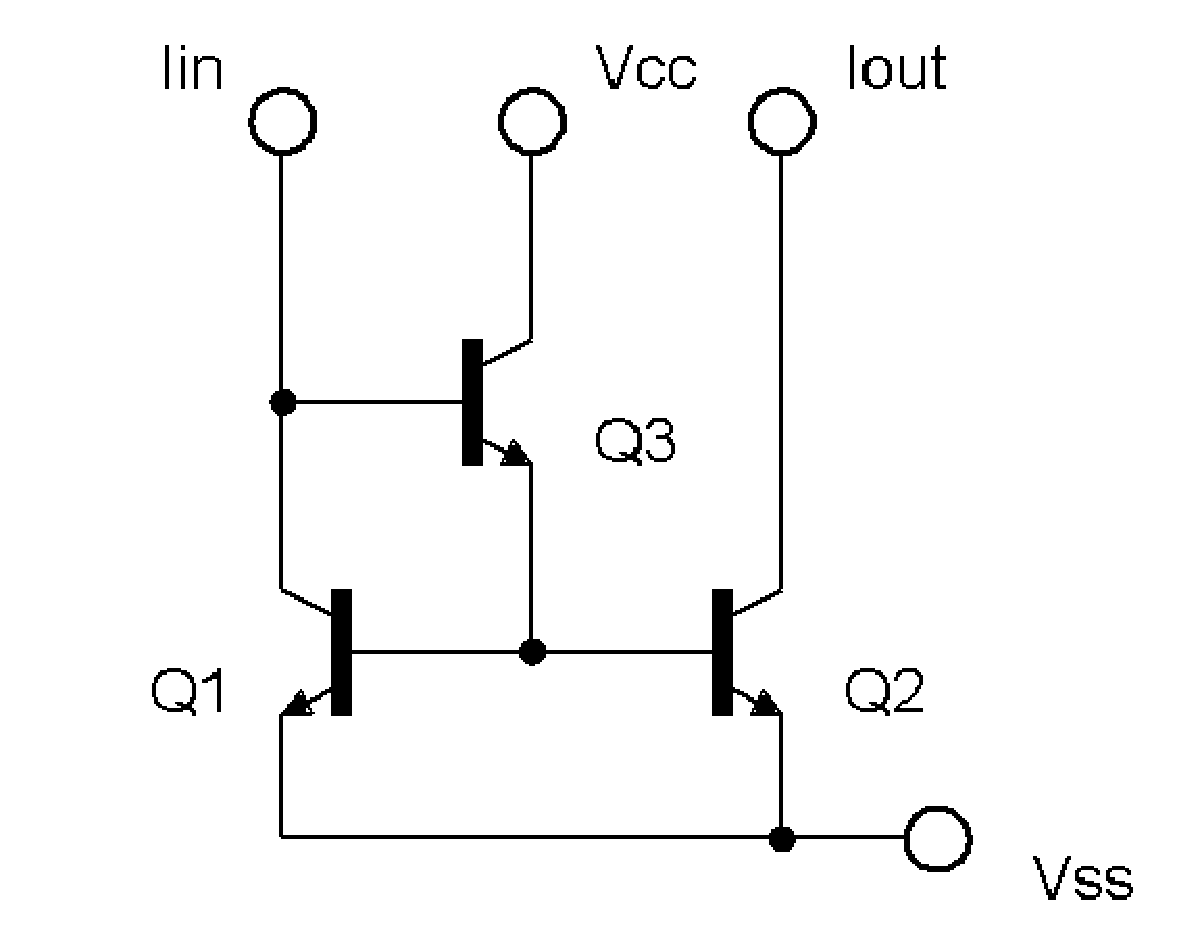
\includegraphics[scale=0.5]{obrazky/ZlepseneWilsonovoZrcadloNPN}
  \end{center}
  \caption{Zlepšené Wilsonovo proudové zrcadlo.}
\end{figure}

Pro sazbu vektorových obrázků přímo v~\LaTeX{}u je možné doporučit balíček \href{https://www.ctan.org/pkg/pgf}{\texttt{TikZ}}.
Příklady sazby je možné najít na \href{http://www.texample.net/tikz/examples/}{\TeX{}ample}.
Pro vyzkoušení je možné použít programy QTikz nebo TikzEdt.




\chapter{Příklad sazby zdrojových kódů}

\section{Balíček \texttt{listings}}

Pro vysázení zdrojových souborů je možné použít balíček \href{https://www.ctan.org/pkg/listings}{\texttt{listings}}.
Balíček zavádí nové prostředí \texttt{lstlisting} pro sazbu zdrojových kódů, jako například:
%
\begin{lstlisting}[language={[LaTeX]TeX}]
\section{Balíček lstlistings}
Pro vysázení zdrojových souborů je možné použít
	balíček \href{https://www.ctan.org/pkg/listings}%
	{\texttt{listings}}.
Balíček zavádí nové prostředí \texttt{lstlisting} pro
	sazbu zdrojových kódů.
\end{lstlisting}
%
Podporuje množství programovacích jazyků.
Kód k~vysázení může být načítán přímo ze zdrojových souborů.
Umožňuje vkládat čísla řádků nebo vypisovat jen vybrané úseky kódu.
Např.:

\noindent
Zkratky jsou sázeny v~prostředí \texttt{seznamzkratek}:
\label{lst:zkratky}
\lstinputlisting[language={[LaTeX]TeX},nolol,numbers=left,firstline=1,lastline=1]{text/zkratky.tex}
%
Šířka textu druhého parametru \verb|KolikMista| udává šířku prvního sloupce se zkratkami.
Proto by měla být zadávána nejdelší zkratka nebo symbol.
Příklad definice zkratky \zk{symfvz} je na výpisu \ref{lst:symfvz}.

\iflanguage{czech}{\shorthandoff{-}}{}
\iflanguage{slovak}{\shorthandoff{-}}{}
\lstinputlisting[language={[LaTeX]TeX},frame=single,caption={Ukázka sazby zkratek},label=lst:symfvz,numbers=left,linerange={bsymfvz-\%\%\%\ esymfvz},includerangemarker=false]{text/zkratky.tex}
\iflanguage{slovak}{\shorthandon{-}}{}
\iflanguage{czech}{\shorthandon{-}}{}

\noindent
Ukončení seznamu je provedeno ukončením prostředí:
\lstinputlisting[language={[LaTeX]TeX},nolol,numbers=left,firstnumber=22,linerange=22]{text/zkratky.tex}

\vspace{\fill}

\noindent
{\bf Poznámka k~výpisům s~použitím volby jazyka \verb|czech| nebo \verb|slovak|:}\newline
Pokud Váš zdrojový kód obsahuje znak spojovníku \verb|-|, pak překlad může skončit chybou.
Ta je způsobená tím, že znak \verb|-| je v~českém nebo slovenském nastavení balíčku \verb|babel| tzv.\ aktivním znakem.
Přepněte znak \verb|-| na neaktivní příkazem \verb|\shorthandoff{-}| těsně před výpisem a hned za ním jej vraťte na aktivní příkazem \verb|\shorthandon{-}|.
Podobně jako to je ukázáno ve zdrojovém kódu šablony.


\clearpage

%\section{Výpis kódu prostředí Matlab}
Na výpisu \ref{lst:priklad.vypis.kodu.Matlab} naleznete příklad kódu pro Matlab, na výpisu \ref{lst:priklad.vypis.kodu.C} zase pro jazyk~C.

\lstnewenvironment{matlab}[1][]{%
\iflanguage{czech}{\shorthandoff{-}}{}%
\iflanguage{slovak}{\shorthandoff{-}}{}%
\lstset{language=Matlab,numbers=left,#1}%
}{%
\iflanguage{slovak}{\shorthandon{-}}{}%
\iflanguage{czech}{\shorthandon{-}}{}%
}

\begin{matlab}[frame=single,float=htbp,caption={Příklad Schur-Cohnova testu stability v~prostředí Matlab.},label=lst:priklad.vypis.kodu.Matlab,numberstyle=\scriptsize, numbersep=7pt]
%% Priklad testovani stability filtru

% koeficienty polynomu ve jmenovateli
a = [ 5, 11.2, 5.44, -0.384, -2.3552, -1.2288];
disp( 'Polynom:'); disp(poly2str( a, 'z'))

disp('Kontrola pomoci korenu polynomu:');
zx = roots( a);
if( all( abs( zx) < 1))
    disp('System je stabilni')
else
    disp('System je nestabilni nebo na mezi stability');
end

disp(' '); disp('Kontrola pomoci Schur-Cohn:');
ma = zeros( length(a)-1,length(a));
ma(1,:) = a/a(1);
for( k = 1:length(a)-2)
    aa = ma(k,1:end-k+1);
    bb = fliplr( aa);
    ma(k+1,1:end-k+1) = (aa-aa(end)*bb)/(1-aa(end)^2);
end

if( all( abs( diag( ma.'))))
    disp('System je stabilni')
else
    disp('System je nestabilni nebo na mezi stability');
end
\end{matlab}

\noindent
\begin{minipage}{\linewidth}


%\section{Výpis kódu jazyka C}

\begin{lstlisting}[frame=single,numbers=right,caption={Příklad implementace první kanonické formy v~jazyce C.},label=lst:priklad.vypis.kodu.C,basicstyle=\ttfamily\small, keywordstyle=\color{black}\bfseries\underbar,]
// první kanonická forma
short fxdf2t( short coef[][5], short sample)
{
	static int v1[SECTIONS] = {0,0},v2[SECTIONS] = {0,0};
	int x, y, accu;
	short k;

	x = sample;
	for( k = 0; k < SECTIONS; k++){
		accu = v1[k] >> 1;
		y = _sadd( accu, _smpy( coef[k][0], x));
		y = _sshl(y, 1) >> 16;

		accu = v2[k] >> 1;
		accu = _sadd( accu, _smpy( coef[k][1], x));
		accu = _sadd( accu, _smpy( coef[k][2], y));
		v1[k] = _sshl( accu, 1);

		accu = _smpy( coef[k][3], x);
		accu = _sadd( accu, _smpy( coef[k][4], y));
		v2[k] = _sshl( accu, 1);

		x = y;
	}
	return( y);
}
\end{lstlisting}
\end{minipage}







\chapter{Obsah přiloženého CD}
Nezapomeňte uvést, co čtenář najde na přiloženém médiu.
Je vhodné okomentovat obsah každého adresáře, specifikovat, který soubor obsahuje důležitá nastavení, který soubor je určen ke spuštění atd.
Také je dobře napsat, v~jaké verzi software byl kód testován (např.\ Matlab 2010b).

Pokud je souborů hodně a jsou organizovány ve více složkách,  je možné pro výpis adresářové struktury použít balíček \href{https://www.ctan.org/pkg/dirtree}{\texttt{dirtree}}.

{\small
%
\dirtree{%.
.1 /\DTcomment{kořenový adresář přiloženého CD}.
.2 loga\DTcomment{loga školy a fakulty}.
.3 FEKT-spec-color.eps.
.3 FEKT-spec-color.pdf.
.3 logolink-op\_vavpi.png.
.3 RE-spec-color.eps.
.3 RE-spec-color.pdf.
.3 SIX\_logo\_zahlavi.png.
.2 obrazky\DTcomment{ostatní obrázky}.
.3 soucastky.eps.
.3 soucastky.png.
.3 spoje.eps.
.3 spoje.png.
.3 ZlepseneWilsonovoZrcadloNPN.eps.
.3 ZlepseneWilsonovoZrcadloNPN.png.
.3 ZlepseneWilsonovoZrcadloPNP.eps.
.3 ZlepseneWilsonovoZrcadloPNP.png.
.2 pdf\DTcomment{pdf stránky generované informačním systémem}.
.3 student-desky.pdf.
.3 student-titulka.pdf.
.3 student-zadani.pdf.
.2 text\DTcomment{zdrojové textové soubory}.
.3 literatura.tex.
.3 prilohy.tex.
.3 reseni.tex.
.3 uvod.tex.
.3 vysledky.tex.
.3 zaver.tex.
.3 zkratky.tex.
.2 navod-sablona\_FEKT.pdf\DTcomment{návod na používání šablony}.
.2 obhajoba.tex\DTcomment{hlavní soubor pro sazbu prezentace k~obhajobě}.
.2 readme.txt\DTcomment{soubor s~popisem obsahu CD}.
.2 sablona.tex\DTcomment{hlavní soubor pro sazbu kvalifikační práce}.
.2 thesis.sty\DTcomment{balíček pro sazbu kvalifikačních prací}.
}
}

\end{document}
